\documentclass[a4paper,portuguese,10pt]{article}

\usepackage{setspace}
\usepackage[hang,footnotesize]{caption}
\usepackage[utf8]{inputenc}
\usepackage{graphicx}
%\usepackage{hyperref}
\usepackage[colorlinks=true]{hyperref}
\hypersetup{
  linkcolor=blue,
  citecolor=blue,
}
%\usepackage{setspace}
%\usepackage{abntcite}
\usepackage{amsfonts}
\usepackage{amsmath}
\usepackage{nonfloat}
\usepackage{semtrans}
\usepackage[margin=2cm]{geometry}
\usepackage[portuguese]{babel}
\usepackage[fixlanguage]{babelbib}
\selectbiblanguage{portuguese}
\usepackage[svgnames]{xcolor} % Specify colors by their 'svgnames'; list of all colors available: http://www.latextemplates.com/svgnames-colors
\usepackage{titlesec}
\usepackage[numbers]{natbib}
\usepackage{nomencl}
\usepackage{ifthen}
\usepackage{multicol} % use of multiple columns
\usepackage{fancyhdr}
\usepackage{draftwatermark}
\SetWatermarkText{PRELIMINAR}
\SetWatermarkScale{3}
%\SetWatermarkColor[rgb]{red!60}
\SetWatermarkLightness{.9}

\columnsep=8mm
%\columnseprule=1pt

\makenomenclature
% no build the list of symbols, use the following command:
% makeindex report_Leon_TUD_02-June.nlo -s nomencl.ist -o report_Leon_TUD_02-June.nls

\onehalfspacing

\newcommand{\p}{\parallel}
\newcommand{\m}{\mid}
\newcommand{\del}{\bigtriangleup}
\newcommand{\lb}{\linebreak}
\newcommand{\nl}{\newline}
%\renewcommand{\div}{{\,\rm div}\,}
\renewcommand{\div}{\nabla\cdot}
%\newcommand{\grad}{\,\rm {grad}\,}
\newcommand{\grad}{\nabla}
\renewcommand{\D}{\partial}
\newcommand{\RR}{\mathbb{R}}
\renewcommand{\vec}{\mathbf}
\newcommand{\esp}{\text{\hspace{2mm}}}
\newcommand{\dgs}{\textordmasculine}
\renewcommand{\max}{\operatorname{max}}
\newcommand{\Ra}{\operatorname{Ra}}
\renewcommand{\Re}{\operatorname{Re}}
\newcommand{\Gr}{\operatorname{Gr}}
\newcommand{\St}{\operatorname{St}}
\renewcommand{\Pr}{\operatorname{Pr}}
\newcommand{\CFL}{\operatorname{CFL}}

%\setlength{\hoffset}{-1cm}
%\setlength{\textwidth}{17cm}
%\setlength{\parskip}{1cm plus4mm minus3mm}
\setlength{\parskip}{2mm}
\setlength{\parindent}{0mm} % Default is 15pt.
\titleformat*{\section}{\normalsize\bfseries}
\titleformat*{\subsection}{\normalsize}

\renewcommand{\refname}{\normalsize{References}}
\renewcommand{\nomname}{List of Symbols}

\renewcommand{\nomgroup}[1]{%
\ifthenelse{\equal{#1}{R}}{\item[\textbf{Roman letters}]}{%
\ifthenelse{\equal{#1}{G}}{\item[Greek letters]}{}}}

\pagestyle{fancy}
\lhead{}
\rhead{\small{Equação de Bernoulli}}

%%%%%%%%%%%%%%%%%%%%%%%%%%%%%%%%%%%%%%%%%%%%%%%%%%%%%%%%%%%%%%%%%%%%%%%%%%
\begin{document}

\thispagestyle{empty}

\begin{minipage}{0.5\linewidth}
\flushleft
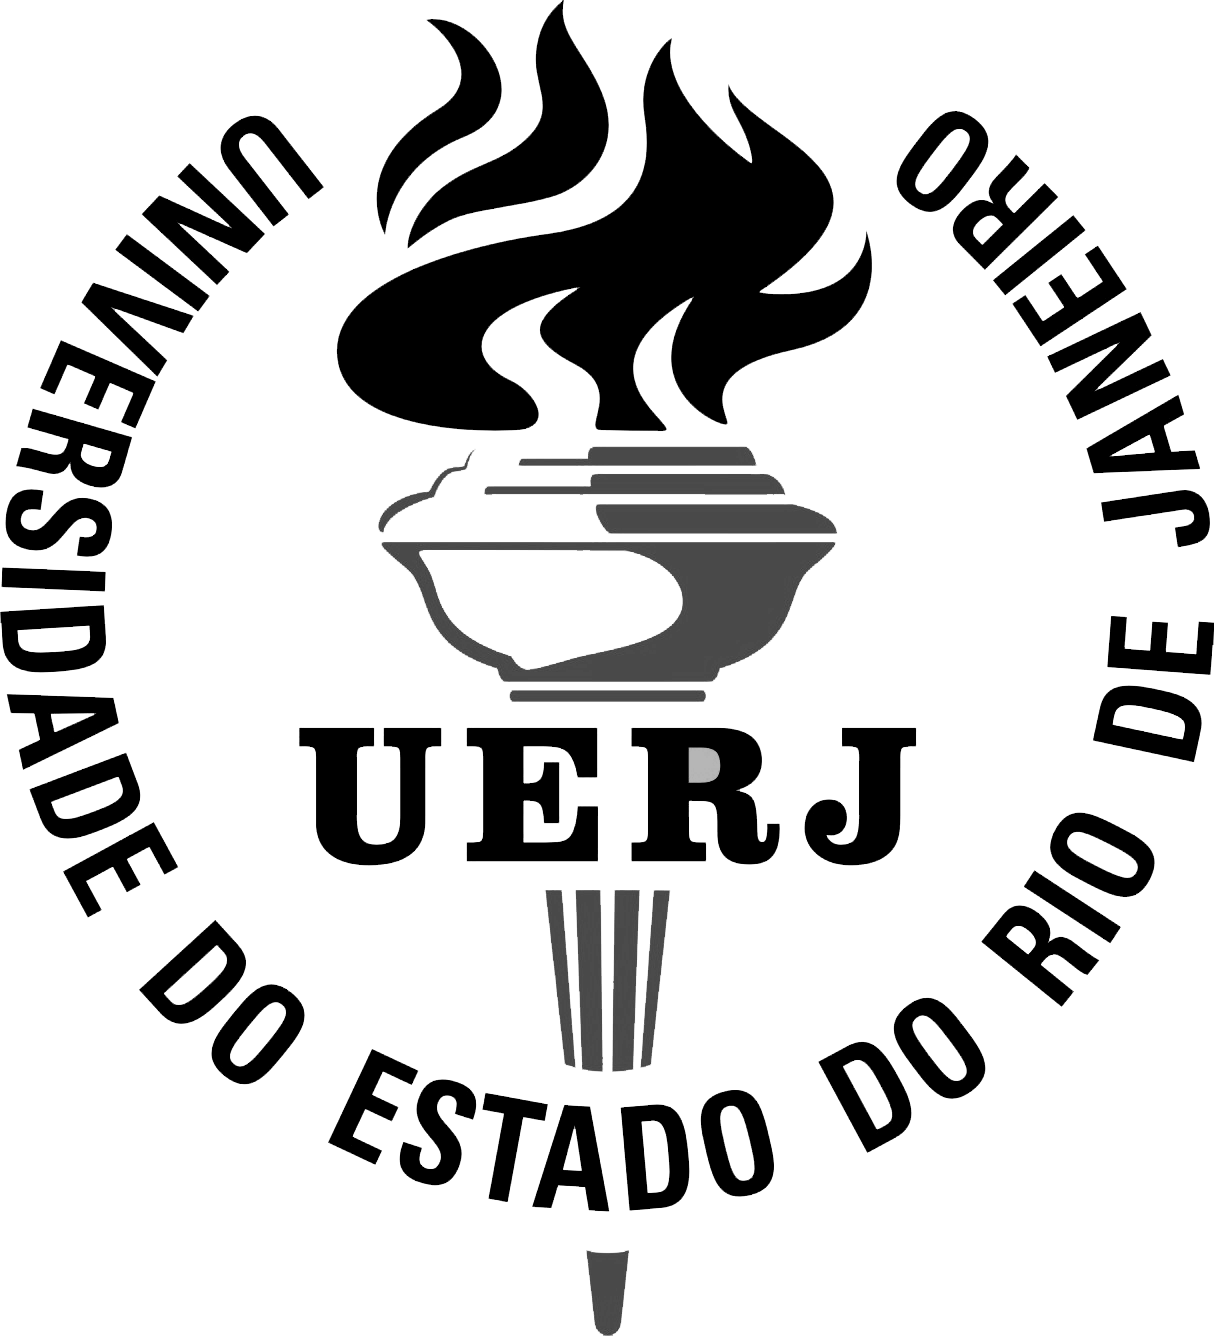
\includegraphics[height=20mm]{./figs/logo_uerj_PB.png}
\end{minipage}
\begin{minipage}{0.5\linewidth}
\flushright

\includegraphics[height=18mm]{./figs/logo_ppg-em.jpg}
\end{minipage}

\hrulefill


%\begin{center}
%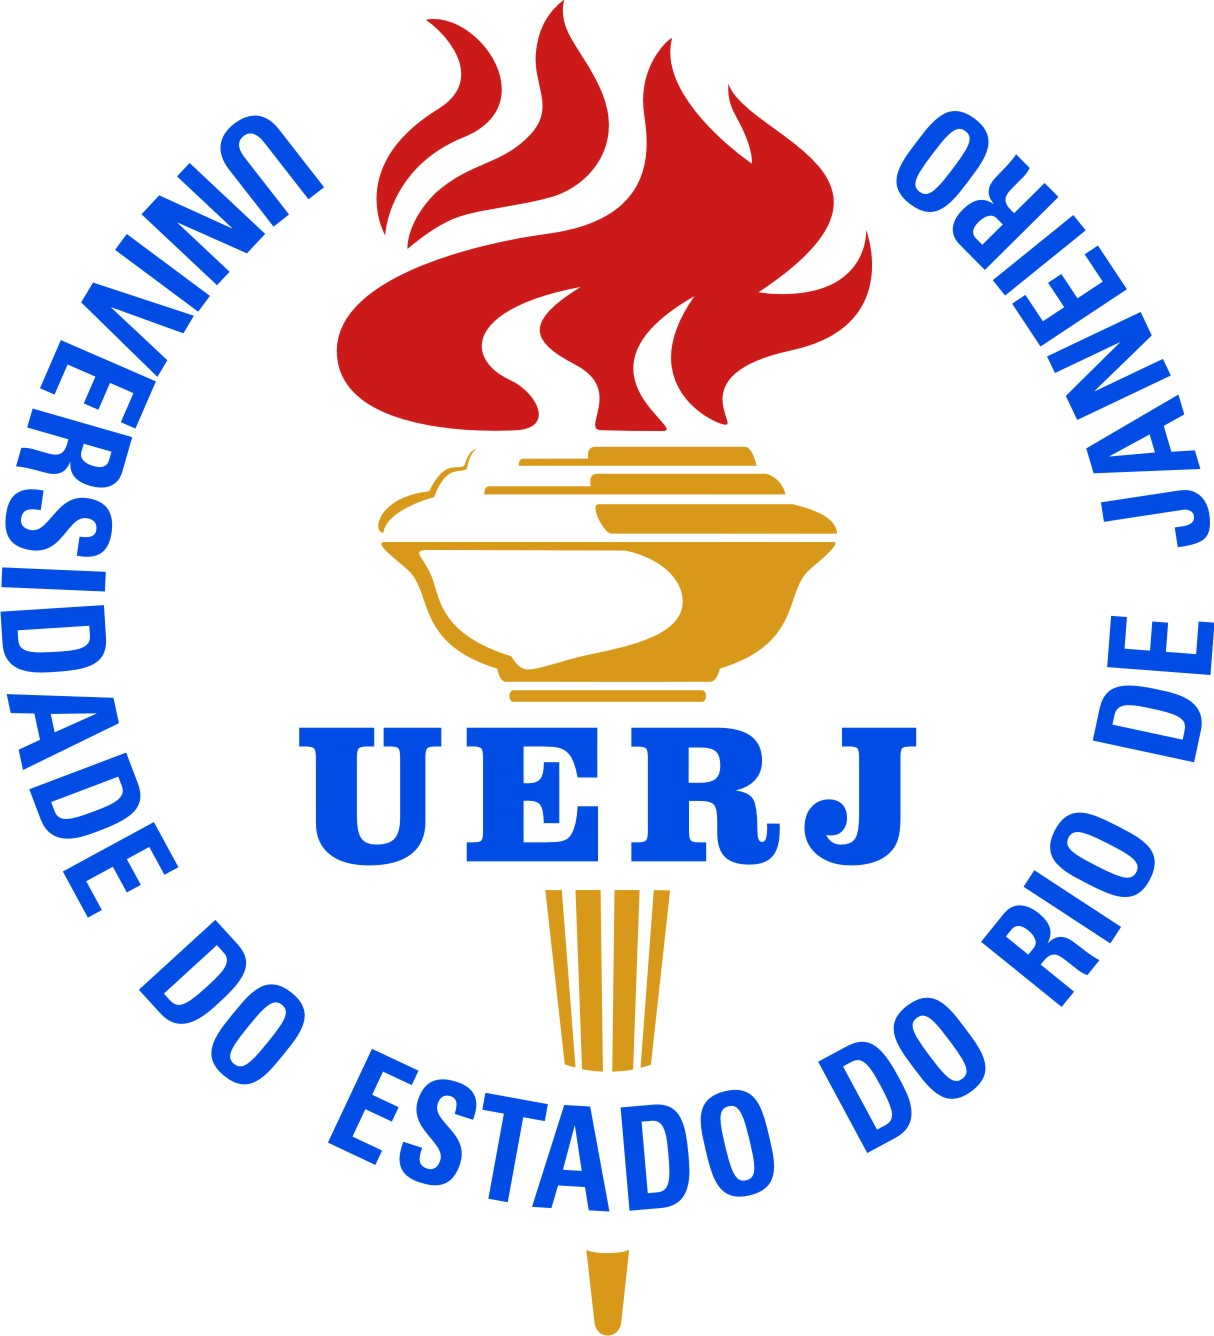
\includegraphics[scale=.3]{../../imagens/logouerj.jpg}\\
%\vspace{5mm}
%{\Large\texttt{Faculdade de Engenharia Mecânica - UERJ}}\\
%\vspace{10mm}
%\end{center}


%\vspace{5mm}
\Large \color{NavyBlue} \textbf{EQUAÇÃO DE BERNOULLI}\\
\color{Black} % Title
\normalsize \texttt{Preparado por: Leon Lima}\\%[0.5cm] % Author(s)
\normalsize \texttt{\today}
\vspace{-2mm}

\setcounter{tocdepth}{1}
\hrulefill\\

Considere as equações de Navier-Stokes para escoamentos compressíveis:

\begin{subequations}
\begin{eqnarray}
  \frac{\D\rho}{\D t} + \div(\rho\vec{v}) &=& 0\\
  \rho\frac{\D\vec{v}}{\D t}+\rho\vec{v}\cdot\grad\vec{v} &=& -\grad P + \div[\lambda(\div\vec{v})\vec{I} + \mu\grad\vec{v}+\mu(\grad\vec{v})^T] + \vec{f}
\end{eqnarray}
\label{eq_ns}
\end{subequations}

Em muitas aplicações de engenharia, é bastante comum ocorrerem escoamentos de fluidos Newtonianos nos quais os efeitos viscosos são desprezíveis em relação aos efeitos de convecção. A conservação de quantidade de movimento para estes escoamentos pode ser modelada pela equação de quantidade de movimento acima desprezando os termos viscosos, ou seja,

\begin{equation}
  \rho\frac{\D\vec{v}}{\D t}+\rho\vec{v}\cdot\grad\vec{v} = -\grad P + \vec{f}
\label{eq_qdm_inviscido}
\end{equation}

Agora, leve em conta a seguinte identidade:

\begin{equation}
  \vec{v}\times\vec{w} = \grad\left(\frac{1}{2}v^2\right) - \vec{v}\cdot\grad\vec{v}
  \label{eq_identidade}
\end{equation}

na qual $\vec{v}\times\vec{w}$ denota o produto vetorial entre $\vec{v}$ e $\vec{w}$, onde $\vec{w} = \nabla\times\vec{v}$ representa o rotacional do campo de velocidade. O escalar $v$ é o módulo da velocidade. É fácil verificar a identidade \ref{eq_identidade} assumindo uma dimensão e expandindo as operações.

Considere agora que a única força de corpo atuante seja a gravidade, ou seja,  $\vec{f} = \rho\vec{g}$, onde $\vec{g}=-g\vec{k}$, sendo $g$ o módulo da aceleração da gravidade (constante) e $\vec{k}$ um vetor unitário com a mesma direção e sentido oposto ao de $\vec{g}$. Assumindo que a coordenada espacial da direção de $\vec{k}$ seja $z$, temos que $\grad(gz) = g\vec{k}$. Ou seja, $\vec{f} = \rho\grad(gz)$.

Inserindo essas considerações na equação \ref{eq_qdm_inviscido}, obtemos

\begin{equation}
  \frac{\D\vec{v}}{\D t} -\vec{v}\times\vec{w} = -\frac{1}{\rho}\grad P - \grad\left(\frac{1}{2}v^2\right) -\grad(gz)
\label{eq_qdm_01}
\end{equation}

É possível observar que todos os termos do lado direito são escritos na forma de gradiente de um campo escalar. A exceção é o termo da pressão, que é multiplicado por $1/\rho$. Será interessante buscarmos uma forma para a equaçao \ref{eq_qdm_01} na qual todos os termos são escritos como gradiente de um escalar. Para tanto, vamos supor que o escoamento seja isotérmico. Se fato, muitos escoamentos de interesse possuem distribuição uniforme de temperatura. Nestes casos, a densidade $\rho$ é função apenas da pressão, o que nos permite escrever

\begin{equation}
  \frac{d}{dP}\int_{P_0}^P\frac{dP}{\rho} = \frac{1}{\rho}
  \label{eq_press_per_dens_01}
\end{equation}

De fato, se definirmos a função $h(P) = 1/\rho$, pelo Teorema Fundamental do Cálculo, temos que

\begin{equation}
  \int_{P_0}^Ph(P)dP = H(P) - H(P_0)
  \label{eq_press_per_dens_02}
\end{equation}

onde $H(P)$ é a primitiva de $h(P)$. Temos, então, que

\begin{equation}
  \frac{d}{dP}\int_{P_0}^P\frac{dP}{\rho} = \frac{d}{dP}\left[H(P)-H(P_0)\right] = h(P) = \frac{1}{\rho}
  \label{eq_press_per_dens_03}
\end{equation}

Dentro demontrado \ref{eq_press_per_dens_01}, podemos escrever

\begin{equation}
  \frac{1}{\rho}\grad P = \left[ \frac{d}{dP}\int_{P_0}^P\frac{dP}{\rho} \right] \grad P
  \label{eq_press_per_dens_04}
\end{equation}

Mas, levando em conta a equação \ref{eq_press_per_dens_02}, e aplicando a regra da cadeia, obtemos

\begin{equation}
  \left[ \frac{d}{dP}\int_{P_0}^P\frac{dP}{\rho} \right] \grad P = \frac{d}{dP}[H(P) - H(P_0)]\grad P = \grad H
  \label{eq_press_per_dens_05}
\end{equation}

o que nos permite concluir que

\begin{equation}
  \frac{1}{\rho}\grad P = \grad\int_{P_0}^P\frac{dP}{\rho}
  \label{eq_press_per_dens_06}
\end{equation}

Com isso, o lado direito da equação \ref{eq_qdm_01} pode ser reescrito em termos do gradiente de um único campo escalar, isto é,

\begin{equation}
  \frac{\D\vec{v}}{\D t} -\vec{v}\times\vec{w} = -\grad\left[ \int_{P_0}^P\frac{dP}{\rho} + \frac{1}{2}v^2 + gz \right]
  \label{eq_qdm_02}
\end{equation}

Introduzimos agora $s$ como sendo um parâmetro ao longo de uma curva qualquer do escoamento. A equação \ref{eq_qdm_02} projetada nessa curva é dada por

\begin{equation}
  \frac{\D\vec{v}}{\D t}\cdot\frac{d\vec{p}}{ds} -(\vec{v}\times\vec{w})\cdot\frac{d\vec{p}}{ds} = -\frac{d\vec{p}}{ds}\cdot\grad\left[ \int_{P_0}^P\frac{dP}{\rho} + \frac{1}{2}v^2 + gz \right] = -\frac{d}{ds}\left[ \int_{P_0}^P\frac{dP}{\rho} + \frac{1}{2}v^2 + gz \right]
  \label{eq_qdm_03}
\end{equation}

onde $\frac{d\vec{p}}{ds}$ é o vetor unitário tangentes à curva no ponto $\vec{p}$. Se essa curva for uma linha de corrente\footnote{Curva formada por todos os pontos nos quais o vetor velocidade é tangente num certo instante do escoamento.}, então, sabendo que $\vec{v}\times\vec{w}$ é ortogonal a $\vec{v}$ e que $\frac{d\vec{p}}{ds}$ tem a mesma direção de $\vec{v}$, temos que $(\vec{v}\times\vec{w})\cdot\frac{d\vec{p}}{ds} = 0$. Além disso, é possível mostrar que

\begin{equation}
  \frac{d}{ds}\int_{s_0}^s\left(\frac{d\vec{v}}{dt}\cdot\frac{d\vec{p}}{ds}\right)ds = \frac{d\vec{v}}{dt}\cdot\frac{d\vec{p}}{ds}
\end{equation}

Com isso, para uma linha de corrente, obtemos

\begin{equation}
 -\frac{d}{ds}\left[ \int_{P_0}^P\frac{dP}{\rho} + \frac{1}{2}v^2 + gz - \int_{s_0}^s\left(\frac{d\vec{v}}{dt}\cdot\frac{d\vec{p}}{ds}\right)ds\right] = 0
  \label{eq_qdm_04}
\end{equation}

Ou seja, podemos concluir que

\begin{equation}
  \int_{P_0}^P\frac{dP}{\rho} + \frac{1}{2}v^2 + gz - \int_{s_0}^s\left(\frac{d\vec{v}}{dt}\cdot\frac{d\vec{p}}{ds}\right)ds = \text{constante}
  \label{eq_bernoulli}
\end{equation}

Esta é a \textbf{equação de Bernoulli}. Ela é válida ao longo de uma linha de corrente para escoamentos onde os efeitos viscosos são muito menores do que os efeitos de convecção e podem, portanto, ser desprezados. Outra hipótese adotada foi a de que o escoamento é isotérmico, ou seja, a densidade é uma função apenas da pressão. \citet{SLATTERY99} mostra ainda que, para escoamentos potenciais, a equação de Bernoulli é válida em todo o domínio do escoamento.

No entanto, essa equação não está na forma como é normalmente vista. Se considerarmos o estado permanente do escoamento ($\D\vec{v}/\D t = 0$), e que a densidade é constante (para água, a pressões baixas, a densidade de fato tem variações muito baixas com a pressão) temos que

\begin{equation}
  \frac{P}{\rho} + \frac{1}{2}v^2 + gz = \text{constante}
  \label{eq_bernoulli_simpl}
\end{equation}

que é a forma popular da equação de Bernoulli. Vamos agora sumarizar as condições para as quais a equação \ref{eq_bernoulli_simpl} é válida:

\begin{enumerate}
  \item fluido newtoniano;
  \item escoamento invíscido\footnote{Escoamentos nos quais os efeitos viscosos são muito pequenos se comparados aos efeitos convectivos.};
  \item densidade constante\footnote{Para a equação completa de Bernoulli \ref{eq_bernoulli} a restrição é de que a densidade é função apenas da pressão.};
  \item válido somente ao longo de uma mesma linha de corrente\footnote{Para escoamentos potenciais, a equação de Bernoulli \ref{eq_bernoulli} é válida em todo o domínio do escoamento \cite{SLATTERY99}.};
  \item estado permanente.
\end{enumerate}

\singlespacing
%\printnomenclature

\bibliographystyle{plainnat}
\bibliography{ref}

\end{document}
